\documentclass{acm_proc_article-sp}
\usepackage{hyperref}

\begin{document}

\title{The Wikipedia Adventure: an Interactive Tutorial for New Wikipedia Users\titlenote{This is a class report for CS 294-78 ("Special topics on Technologies for Education and Learning at Large Scale") and SCMATHE 220c ("Science and Mathematics Education: Designing  Educational Technologies") at University of California, Berkeley created in Spring 2012.  All rights are waived under the Creative Commons Zero Waiver (CC0). This is not a peer-reviewed work.}}

\numberofauthors{1}
\author{
\alignauthor
Derrick Coetzee \\
       \affaddr{University of California, Berkeley}\\
       \affaddr{Berkeley, California, USA}\\
       \email{dcoetzee@eecs.berkeley.edu}
}

\maketitle

\begin{abstract}
New contributors to Wikipedia face daunting technical and social challenges, contributing to ongoing decline in editor retention and systemic bias in article content. The Wikipedia Adventure is a web-based interactive tutorial for new users that leads them through learning essential basics in a safe game-like environment, and can extend to instruction on advanced skills. All interactions are tracked and linked to the user's real Wikipedia account, where their performance can be evaluated based on contribution logs. It is currently under development and early evaluation.
\end{abstract}

% A category with the (minimum) three required fields
% \category{H.4}{Information Systems Applications}{Miscellaneous}
%A category including the fourth, optional field follows...
% \category{D.2.8}{Software Engineering}{Metrics}[complexity measures, performance measures]
% \terms{Theory}
% \keywords{ACM proceedings, \LaTeX, text tagging} % NOT required for Proceedings

\section{Motivation}

Since 2007, Wikipedia has experienced declining editor participation and retention, as shown in Figure~\ref{fig:retention}. Suh\cite{Suh:2009} cites ``exclusion of newcomers and resistance to new edits'' as possible explanations. Personal experience shows new editors often either can't figure out how to edit Wikipedia, or have negative experiences due to their unfamiliarity with the site and its policies, and stop editing. Learning policy thoroughly is an overwhelming prospect---just the key policies and guidelines fill a 270-page book---and there is little guidance regarding which policy is most important to learn first. The goal of this project is to help new Wikipedia users to generate quality content by using an interactive, web-based tutorial to teach basic Wikipedia editing and policies.

\begin{figure}
\centering
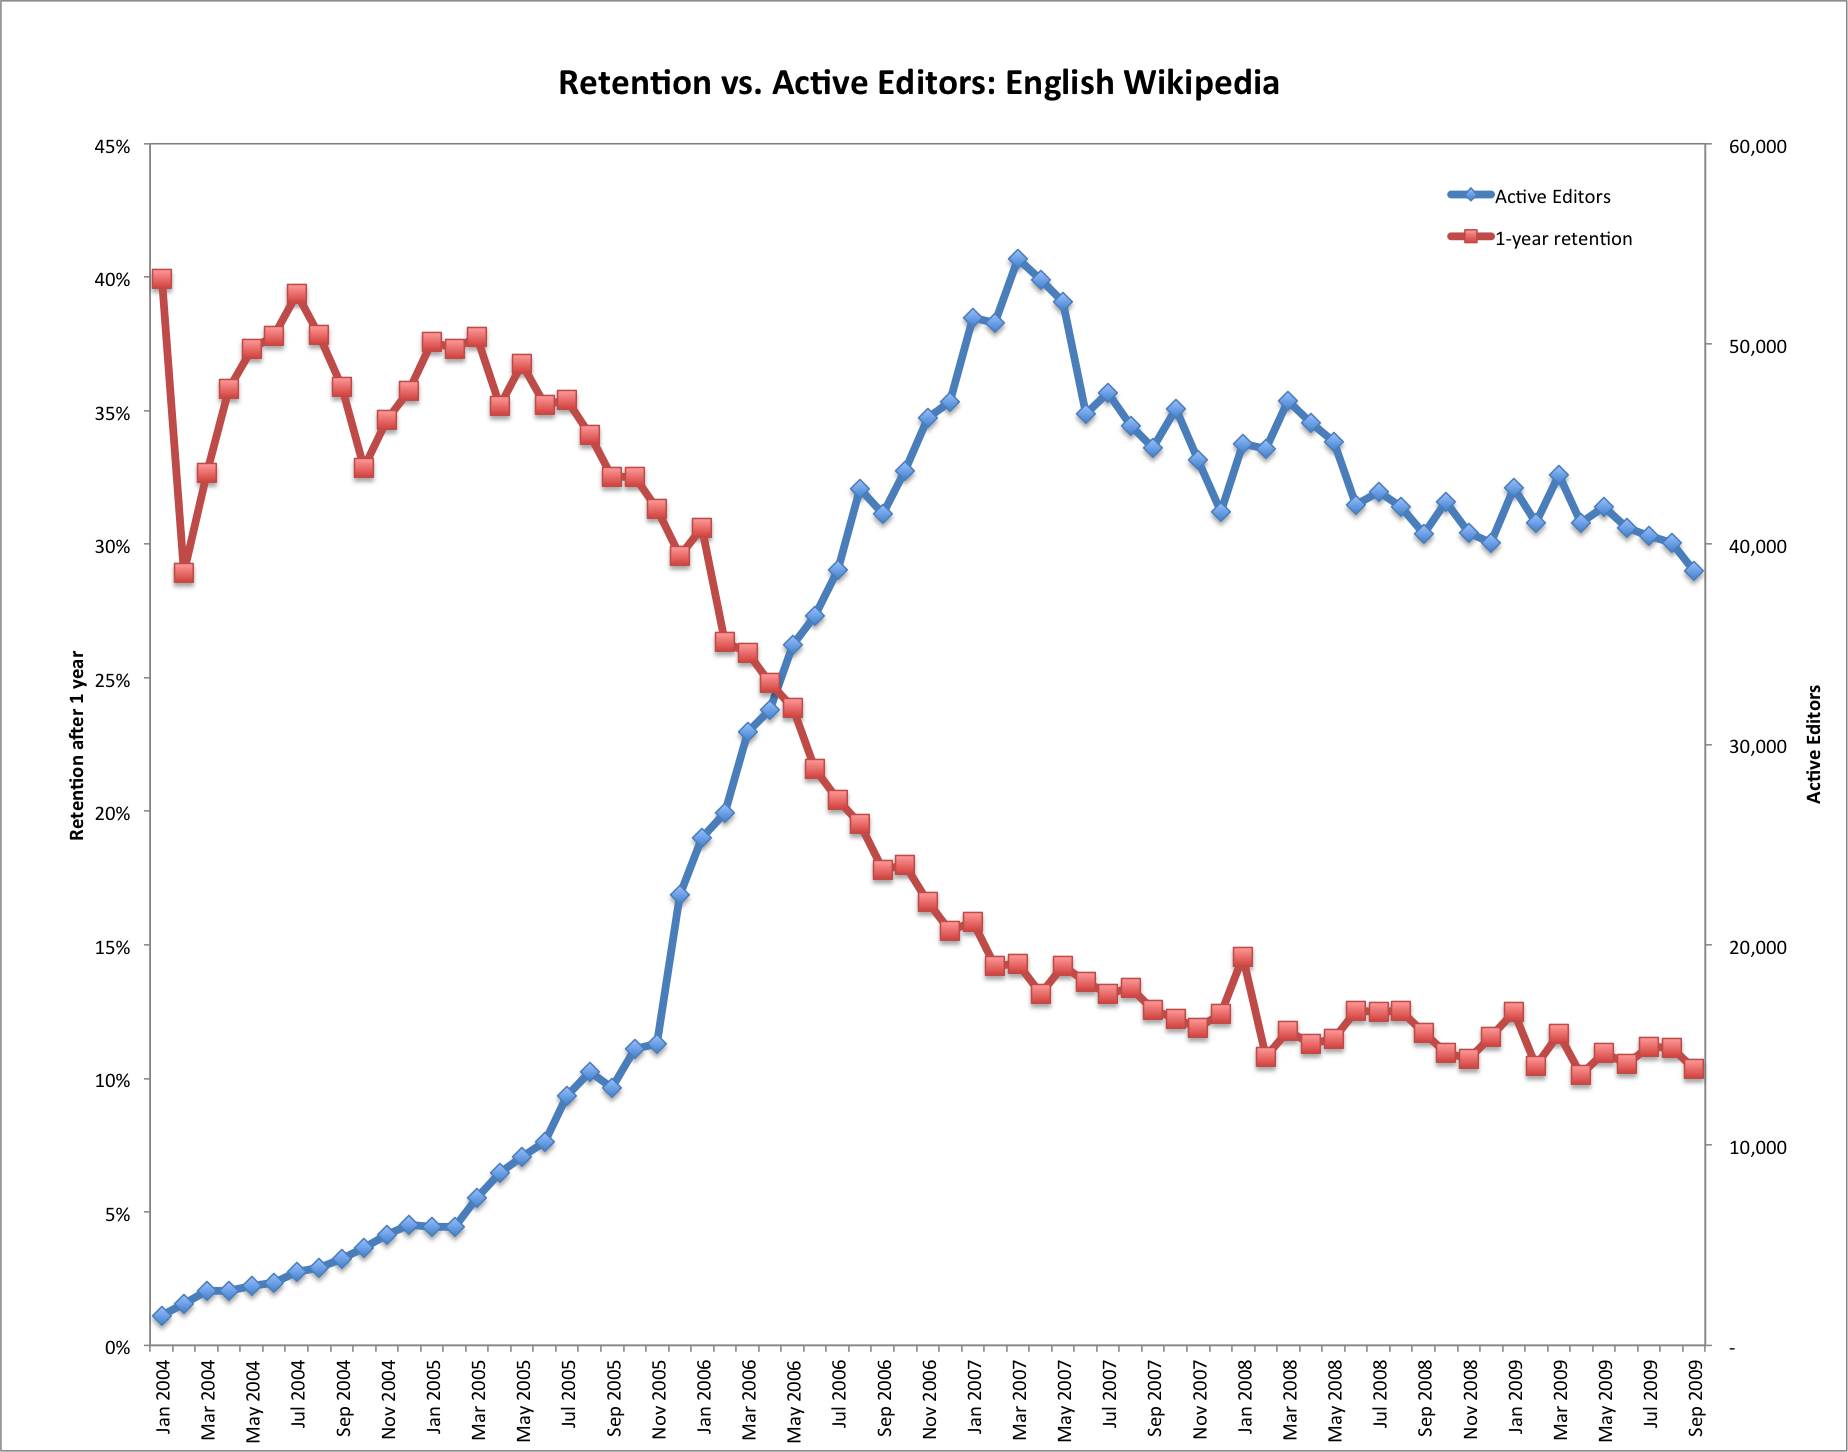
\psfig{file=images/Enwp_retention_vs_active_editors.png, width=\columnwidth,}
\caption{Active editors and editor retention, 2004-2009. Active editors peaked in early 2007 and the one-year editor retention rate has fallen to 10\%. Source: Wikimedia Foundation Editor Trends Study.  
\url{http://strategy.wikimedia.org/wiki/File:Enwp_retention_vs_active_editors.png}}
\label{fig:retention}
\end{figure}

\begin{figure*}
\centering
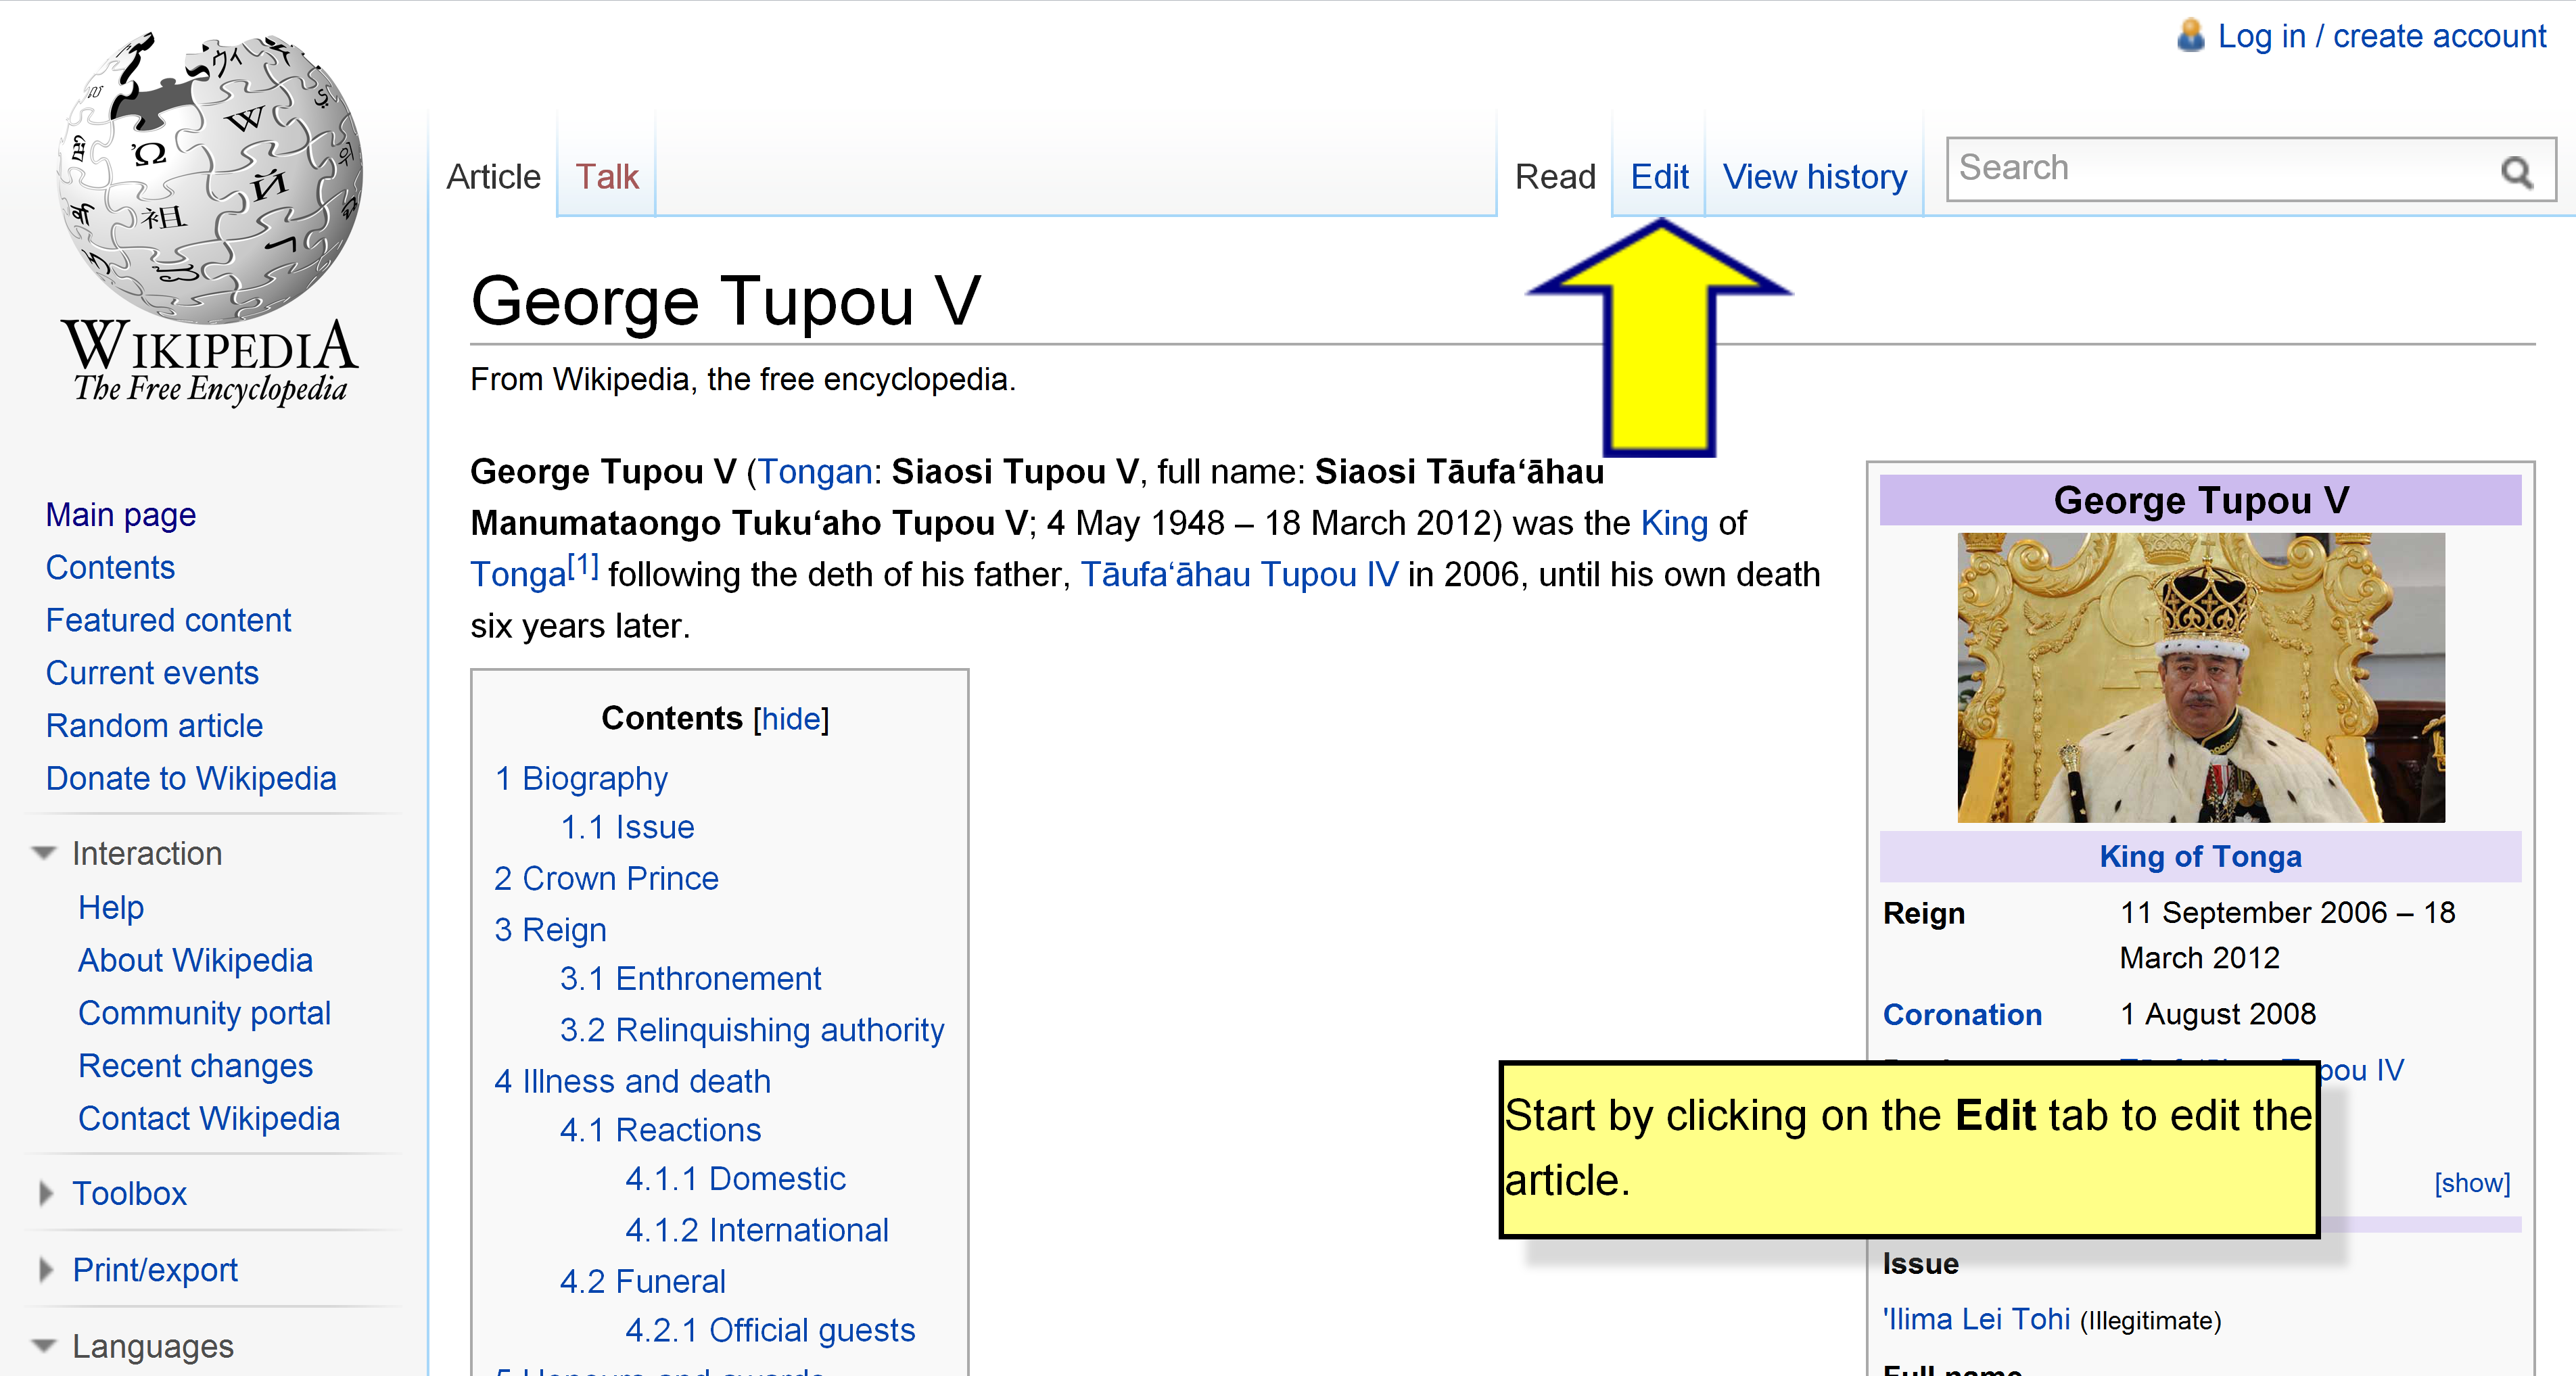
\psfig{file=images/wikipedia_adventure_big.png, width= 2 \columnwidth,}
\caption{Screenshot from first level of The Wikipedia Adventure. The interface is identical in appearance to the real Wikipedia interface, except that instructions are overlaid instructing the user to click on the edit button. }
\label{fig:screenshot}
\end{figure*}

From a user perspective, the motivation to contribute to Wikipedia can come from many sources. Some are financially motivated, seeking to generate publicity for their business, band, or professional works, or to increase web traffic to their website via links. Some are egotistically motivated. Some are students participating as a course requirement. Some are motivated by a desire to ensure articles are accurate, or to spread awareness of a topic or point of view. Some are motivated by a desire to make an impact, some by a desire to attain status in the Wikipedia community, and some by a desire to spread knowledge to others. Motivations of Wikipedia editors have been explored by numerous researchers; a good source is Kuznetsov,\cite{Kuznetsov:2006} which qualitatively explored a number of intrinsic and extrinsic motivating factors such as altruism, reciprocity, community, reputation, and autonomy.

Likewise, the demographics of new Wikipedia users are diverse, coming from all age groups and all regions of the world. Thirteen-year olds in the US routinely contribute to articles on popular culture, and retiree professors abroad who are speakers of English as a second language contribute as experts in their fields. Some carry PhDs in computer science, while others are barely capable of using a web browser. Glott\cite{Glott:2010} gives a survey of Wikipedia user demographics.

Teaching effective Wikipedia editing to such a diverse audience is a challenge: major differences in educational backgrounds and technical skill mean that tasks which are remedial for one audience (such as account creation) are challenging for others. This means the tutorial must be flexible enough to allow users to learn about basic tasks without boring more adept users. The primary strategy used to address this is allowing skipping of early lessons based on answers to questions (for example, users who already have an account are not instructed how to create one).

Another challenge is that many of the motivations listed above are short-term, in the sense that they just want to write a single article (e.g. on their company) or fix a single problematic article and are not interested in investing time and effort in the lessons needed to become a good long-term contributor. Unlike in a classroom environment, users cannot be compelled to complete the tutorial. An effective tutorial must recognize this by teaching the bare essentials needed for a contributor to begin achieving their immediate goal before they lose interest, but also encourage them to return when they encounter new barriers. One way to encourage return is to give a preview of what is taught by future lessons before they depart; another is to place links to lessons on Wikipedia, in the context where they are most useful.

\section{Existing educational resources}

One way for new users to learn to use Wikipedia is to simply start using Wikipedia; this is explicitly encouraged by Wikipedia's ``be bold'' guideline. Upon encountering difficulties, they receive feedback from other users (see Figure~\ref{fig:talktemplate}), consult help pages, ask for help, and experiment. If their understanding is incomplete, they receive further feedback when attempting the task again. Because learning is motivated by successful completion of the task immediately at hand, this facilitates in-context learning that is targeted and personally relevant in the sense of Olfman.\cite{Olfman:1991}

\begin{figure}
\centering
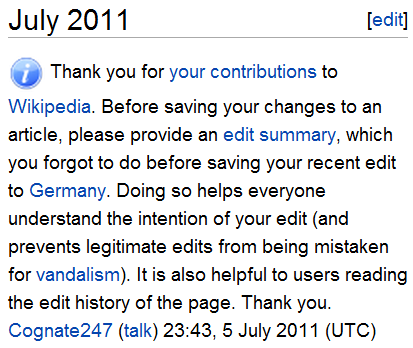
\psfig{file=images/talk_page_message.png, width=2.5 in,}
\caption{A standardized talk page message reminding a user to enter edit summaries when editing. Feedback from other users provides targeted in-context learning, but is costly.}
\label{fig:talktemplate}
\end{figure}

These mechanisms can be highly effective for experienced users who know which of these resources to exploit and at what times, but for new users, these resources are either difficult to locate, difficult to use, or too many options are offered, leading to confusion. Moreover, the written help pages are not interactive, forcing users to experiment on the live site in order to "test out" what they have learned. Some users cause damage, while others, fearing they will break something, are reluctant to experiment, especially in complex articles using sophisticated markup.

Personalized feedback is costly. All new users repeatedly encounter the same issues. Experienced users have resorted to using impersonal standardized messages (\emph{templates}) to provide feedback, as shown in Figure~\ref{fig:talktemplate}. 

Help and policy pages on Wikipedia, like articles, are structured as a web: each one links to many other help and policy pages. While valuable for exploratory learning for long-term users, new users who just want to learn enough to complete their short-term task are frustrated by this, not knowing which of the many linked documents will help them complete the task at hand correctly.

Another limitation of the standard interface is that the main encyclopedia is already well-developed. Notari,\cite{Notari:2006} on motivating students to participate in class wikis, emphasizes the need for a ``launch activity'' which is ``motivating, easy , and quickly achievable.'' Most substantive article-writing activities no longer fall under this description, necessitating the invention of artificial tasks. Although not as motivating as real activities, artificial tasks in a fake environment can be repeated by each user uniformly without consequences, and may be simpler than corresponding tasks on the real project.

\section{Design and learning goals}

The proposed tutorial would simulate the experience of the real Wikipedia website, but not affect the real site, and so is ``insulated from real consequences.'' \cite{Garris:2002} Instead of a complex web of pages, users will be given scripted instructions and a limited number of options at each point, with a mostly linear flow (links/options that are permitted are highlighted, while other links/options are nonfunctional).

The goals of the initial lessons are to help the user learn enough to complete their desired short-term task successfully, while also teaching them enough to seek additional help as needed, either through additional lessons or through existing channels on Wikipedia. As emphasized by Olfman,\cite{Olfman:1994} it's important for initial training to include a combination of procedural training (technical how-to information) and conceptual training (helping new users to build a mental model of the site). In particular, basic concepts like how articles are communally edited and their content determined by consensus are essential for all users to understand.

After completing the initial lessons, which would introduce basic editing and help tools and share a linear narrative, the user would have the option of choosing from a pool of largely independent advanced lessons. These lessons serve two purposes: they allow users interested in exploratory learning and becoming long-term users to continue learning about subjects that interest them, and they allow users who have trouble in a particular area to learn more about that area. In both cases, they help developing editors to become expert, long-term users. By allowing direct web links to lessons, other users can suggest particular lessons, and help pages can link to related lessons. For particularly complex topics, prerequisites can be implemented where one lesson is recommended or required to be completed before another.

The practice of having an initial, easy linear stage followed by a ``wide open'' exploratory space of more difficult stages is common in games, such as in the Final Fantasy series, where players are initially ``railroaded'' along a linear set of locations while learning the mechanics of the game, but are eventually given access to an airship that allows any location in the world to be easily visited in any order.

At certain stages, the user will need to enter text, which needs to be evaluated for compliance to policies, such as "neutral point of view." Because it's not technically feasible to perform this evaluation on arbitrary text, the user would instead be presented a small number of text options, and the option they select is entered for them.

Following success on the English-language Wikipedia, the system would undoubtedly be translated and modified to suit other language Wikipedias, and must be implemented with this in mind.

Negative feedback is a controversial issue. On the real Wikipedia, users receive negative feedback for violating rules, eventually being blocked from editing entirely. The tutorial needs to illustrate that negative actions have negative consequences, without inadvertently encouraging negative actions. There are a couple ways to accomplish this: one is to show others receiving negative feedback in response to negative actions, and another is to give rapid feedback, immediately pointing out the negative action and ask the user to try again.

The initial lessons are of special note because although all new users have a need for certain basic skills, differences in motivation and background may justify altering the approach. Tech-savvy users should be able to skip easy lessons, or else they will be bored and lose interest.  Financially motivated users may need instruction on the conflict of interest policy, whereas altruistic users require none. Lessons can be made more personally relevant, again in the sense of Olfman\cite{Olfman:1991} by using example content in the area of interest of the new user.

\section{Collaboration}

The tutorial described so far merely simulates communication between users, and is not effective at teaching real collaboration. Notari,\cite{Notari:2006} describing use of wikis in constructivist classrooms, places a heavy emphasis on collaboration, from the beginning developing a ``communication and comment culture '' with simple activities like commenting on one another's personal introductions.

One way to address this is to exploit the existing collaborative platform by directing students to complete on-wiki tasks such as creating a real user page or giving feedback on an article talk page before they are permitted to continue to the next lesson, creating a hybrid tutorial experience. Another is to feature interaction among concurrent players.

\section{Drawing users in with game mechanics}

One important goal is to draw users in to the lessons, encouraging them to complete more of them rather than abandon the interaction. A variety of familiar game mechanics can be leveraged for this. Lessons can contain links to related lessons at the end of lessons, encouraging exploratory learning, and players can receive awards for completing lessons (based on number or perhaps for completing a group of related lessons). By displaying awards on the user's real Wikipedia user page, they are motivated by community status. A "high scores" chart comparing their performance to that of other community members may also be motivating. Mandatory prerequisite structures can act as an incentive: a player who wants to complete a particular lesson (perhaps because a special award is attached to it) will go through the necessary prerequisite lessons first, a process known in games as "unlocking."

Another interesting mechanic would be for players to complete certain tasks on the real Wikipedia, and receive "credit" inside the game for it, raising their score or unlocking additional lessons. This would act as a gentle push for users reluctant to make the jump from a safe environment to one with real consequences.

Another important goal is to encourage players to redo lessons that they may not have fully understood the first time. Drawing on games, one way to do this is with a score system that yields the most points for making good editing decisions. To make achieving the best score more challenging, available responses can be chosen randomly each time.

Paras\cite{Paras:2005} emphasizes the importance of incorporating periods of reflection into gameplay, since players do not normally reflect while in a state of flow. In games like Starcraft, this is accomplished by rich visualizations and replays of what occurred during the game that can be reviewed between games. Likewise, if our tutorial possesses a score system, it should allow a player to revisit their responses and where they gained and lost points between lessons, allowing them to identify areas for improvement. This will also create what Garris\cite{Garris:2002} refers to as a ``judgment-behavior-feedback loops,'' an essential advantage of games over passive instruction.

\section{Limitations for initial implementation}

Because the scope of this project is too large for a single-semester course project, choices must be made regarding which part to complete first. A best practice in software scheduling is to target high risk parts of the design first, those that may or may not be successful and/or feasible.\cite{Boehm:1988} There are two main risks that need to be targeted: the technical risks associated with implementing the interface, score system, and review system; and the risk that the system as a whole may not be motivating, engaging, or teach the intended material well.

There is little doubt that, given a few fully-constructed lessons, many similar lessons could be constructed in essentially the same manner, so that spending time on content generation beyond that needed for a basic educational evaluation would be a poor investment. Prototyping the primary tutorial interface is essential. Easy-to-implement features with high payoff, like skipping of easy lessons or placing awards on real user pages, can also be implemented. More sophisticated features like customizing the experience for users with particular interests or motivations have a poorer cost/benefit ratio and can be postponed, as can the advanced lesson pool.

\section{Implementation}
In order to be broadly accessible to the diverse user base of Wikipedia, who already has web access, a web-based tutorial is intuitively advantageous. Running portably across major platforms and on hardware with poor performance is essential. Although some users only access Wikipedia from mobile devices, the editing interface on mobile devices is not usable at the present time, and so a mobile tutorial is unnecessary.

Implementing the tutorial will be challenging, largely because it needs to simulate the already-complex interface of Wikipedia itself, and remain up-to-date as that interface is modified. Major changes to the editing interface, for example,  are planned in the next year. One approach to mitigating this is to base the tutorial on MediaWiki, the open source software used by Wikipedia, with other elements added on top using Javascript. The interface would appear identical to how the user would see it on the real website. Another approach is to use Adobe Flash with screenshots of the actual Wikipedia interface which are updated as needed, which would add versatility and simplify implementation of other elements such as animations at the expense of accurate rendering of the interface.

Although it is intuitively appealing to integrate the tutorial into the main Wikipedia site, making it easily accessible and allowing more interaction between it and the real site, this also risks compromising the impression of safety offered by a clear simulation.

\section{User testing and assessment}
As with any software tool, the most valuable feedback comes from real users. The system must be instrumented to track actions and progress by users, and follow-up surveys or interviews can yield qualitative feedback. By tying users to their Wikipedia user accounts, their performance in the lessons can be correlated with their contribution history as editors. Testing is expected to be an indefinitely ongoing process alongside real use.

New users can be recruited from a variety of existing venues that already deal with new users and answer their questions, including online chat, the Articles for Creation process, welcome messages, and the help desk page. Links can be added to the tutorial where suitable, and volunteers who deal with new users can be trained to link to relevant tutorial lessons over time.

\section{Lesson builder}

A vital component going forward will be to enable users who are not technically savvy to contribute new lessons to the lesson pool. This will dramatically increase breadth and depth of content, motivate recruiting, and allow content creators to learn by teaching. However, this also risks creating the same excess of options presented by the original website, particularly if multiple lessons cover the same topic. One way to address this is to leverage ratings by players to choose their favorite lessons, and display highly-rated lessons in each category at the top.

\section{Conclusions}

\section{Acknowledgments}
The Wikipedia Adventure is based originally on an idea and
initial design defined by User:Ocassi. Mock-ups
were done by User:Sonia. Several
other Wikipedia users and the staff of
CS 294-78 and SCMATHE 220c gave feedback following
review of the design and ad hoc testing.

\bibliographystyle{abbrv}
\bibliography{sigproc}  % sigproc.bib is the name of the Bibliography in this case

\end{document}
